% presentation
\documentclass{beamer}

% \usetheme{Boadilla}
\usetheme{CambridgeUS}
\usecolortheme{dolphin}

% rus lang
\usepackage[main=russian,english]{babel}

% insert images
\usepackage{wrapfig}
\usepackage{graphicx}
\usepackage{float} % для позиционирования изображений
\usepackage{caption}
\captionsetup{format=hang,labelsep=period}
\graphicspath{{./images/}}

% tables
\usepackage{array} % расширенные возможности для работы с таблицами
\usepackage{tabularx} % автоматический подбор ширины столбцов
\usepackage{dcolumn} % выравнивание чисел по разделителю
\usepackage{{booktabs}}

% math
\usepackage{amsmath}
\usepackage{mathtools}
\usefonttheme[onlymath]{serif}
\newtheorem{rustheorem}{Теорема}

\newcommand{\at}[2][]{#1|_{#2}}
\newcommand{\eps}{\varepsilon}
\newcommand{\dd}[2]{\frac{\partial #1}{\partial #2}}

\DeclareMathOperator*{\argmin}{argmin}
\DeclareMathOperator{\sign}{sign}
\DeclareMathOperator{\K}{K}
% \DeclareMathOperator{\R}{\mathbb{R}}
\DeclareMathOperator{\X}{\mathbb{X}}
\DeclareMathOperator{\Y}{\mathbb{Y}}
% \DeclareMathOperator{\E}{\mathbb{E}}
\DeclareMathOperator{\V}{\mathbb{V}}

\newcommand{\E}[1]{\mathbb{E}\left[#1\right]} % Мат ожидание
\newcommand{\D}[1]{\mathbb{D}\left[#1\right]} % Дисперсия
\newcommand{\COV}[2]{\textbf{Cov}\left(#1, #2\right)}
\newcommand{\Cov}{\textbf{Cov}}
\newcommand{\R}{\mathbb{R}}
\renewcommand{\epsilon}{\varepsilon}
\renewcommand{\phi}{\varphi}
% algorithms
\usepackage[]{algorithm2e}

\title[]{МОДЕЛИ ДОХОДНОСТЕЙ АКТИВОВ В СРЕДНЕ-ДИСПЕРСИОННОМ АНАЛИЗЕ МАРКОВИЦА НА КРИПТОВАЛЮТНЫХ РЫНКАХ}
\subtitle{}
\author{Полузёров Т. Д.}
\institute{БГУ ФПМИ}
\date{}

\begin{document}
\begin{frame}
    \titlepage
\end{frame}

\begin{frame}
    \begin{center}
        \frametitle{Структура работы}
        \tableofcontents
    \end{center}
\end{frame}

\section{Портфельная теория}

\begin{frame}
    \frametitle{Однопериодная задача инвестирования}
    Доступны $N$ активов.
    $S_i^0, S_i^1$ --- цены $i$-го актива в моменты времени $t=0$ и
    $t=1$ соответсвенно.

    Доходность актива за период
    \[
        r_i := \frac{S^1 - S^0}{S^0}, i=\overline{1, N}
    \]

    Необходимо сформировать портфель
    \[
        b = (b_1, \dots, b_N)
    \]
    где $b_i$ --- число преобретаемых активов $i$-го типа.

    Портфель покупается в момент $t=0$ и продается в момент $t=1$ по рыночным ценам.
\end{frame}

\begin{frame}
    \frametitle{Требования к портфелю}
    Пусть инвестор имеет капитал $x$.

    Перейдем к долям инсвестирования капитала $x$ в доступные активы.
    \[
        \omega_i := \frac{b_i S_i^0}{x}, i=\overline{1, N}
    \]

    Цена портфеля в момент времени $t=0$
    \[
        X^0 = x
    \]
    В момент $t=1$
    \[
        X^1 = (1+R)X^0 = \sum_{i=1}^{N} \omega_i r_i = \omega^T r
    \]
    где $R$ --- доходность порфтеля
\end{frame}

\begin{frame}
    Предположим что случайные величины доходностей $r_i, i=\overline{1, N}$ известны, тогда
    матожидание и дисперсия случайной величины доходности портфеля равны
    \[
        \mu_X := \E{R} = \sum_{i=1}^{N} \omega_i \E{r_i} = \omega^T \mu
    \]

    \[
        \sigma_X^2 := \sum_{i=1, j=1}^{N} \omega_i \omega_j \COV{r_i}{r_j} =
        \omega^T \Sigma \omega
    \]
    где $\mu = \E{r}$, а $\Sigma$ --- ковариационная матрица случайного вектора $r$.
\end{frame}

\begin{frame}
    \frametitle{Оптимизационная задача}
    Введем параметр $\tau \in [0, +\infty)$ --- толерантность к риску и сформурируем критерий оптимальности
    \[ 
        f(\mu_X, \sigma_X^2) = \tau \omega^T \Sigma \omega - \omega^T \mu \rightarrow \min_{\omega}
    \]

    Оптимизационная задача имеет вид
    \begin{align*}
        \begin{cases}
            \tau \omega^T \Sigma \omega - \omega^T \mu \rightarrow \min_{\omega} \\
            \omega^T e = 1 \\
            \omega \ge 0
        \end{cases}
    \end{align*}

    При $\tau=0$ имеем портфель максимальной доходности, при $\tau \rightarrow +\infty$
    --- минимального риска.
\end{frame}

\section{Методы оценки характеристик доходностей}

\begin{frame}
    На практике в момент времени $t=0$ случайные величины доходностей $r$ неизвестны.
    
    Необходимо оценить характеристики $\hat{\mu}_X$ и $\hat{\Sigma}$.

    Известные подходы:
    \begin{itemize}
        \item Модель CAPM (Capital Asset Pricing Model), У. Шарп, Дж Линтер
        \item Теория  APT (Arbitrage Pricing Theroy), С. Росс, Р. Ролл.
    \end{itemize}
    
    Предлагается иной подход --- применить методы машинного обучения и модели временных
    рядов для решения задачи регрессии по историческим данным.
\end{frame}

\begin{frame}
    \frametitle{Линейная регрессия}
    Пусть $X$ --- матрица объектов-признаков, где признаки это лаги ряда,
    $y$ --- соотвествующие истинные доходности.
    $\theta = (\theta_0, \dots, \theta_k)$ --- параметры.
    
    \[
        a(x) = \theta_0 + \theta_1 x_1 + \dots + \theta_k x_k
    \]
    Оптмальные веса $\theta^*$ методом наименьших квадратов
    \[
        Q(a) = || X\theta - y||^2 \rightarrow \min_{\theta}
    \]
\end{frame}

\begin{frame}
    \frametitle{Случайный лес}

    
\end{frame}

\begin{frame}
    \frametitle{ARIMA}
    
\end{frame}

\section{Проверка статегий на реальных данных}

\begin{frame}
    \frametitle{Входные данные}
    Общие характеристики данных:
    \begin{itemize}
        \item Криптовалютная биржа OKX. 
        \item 8 наиболее популярных активов
        \item Временной период с 1 января 2022 по 1 января 2025.
        \item Дневной таймфрейм
        \item Период инвестирования --- 1 неделя
    \end{itemize}

    Проведение тестирования:
    \begin{itemize}
        \item Данные до 1 января 2024 используются для подбора числа лагов и 
        гиперпараметров моделей
        \item Тестирование проводится на данных за 2024 год
    \end{itemize}
\end{frame}

\begin{frame}
    \begin{columns}
        \begin{column}{0.5\textwidth}
            \begin{figure}
                \centering
                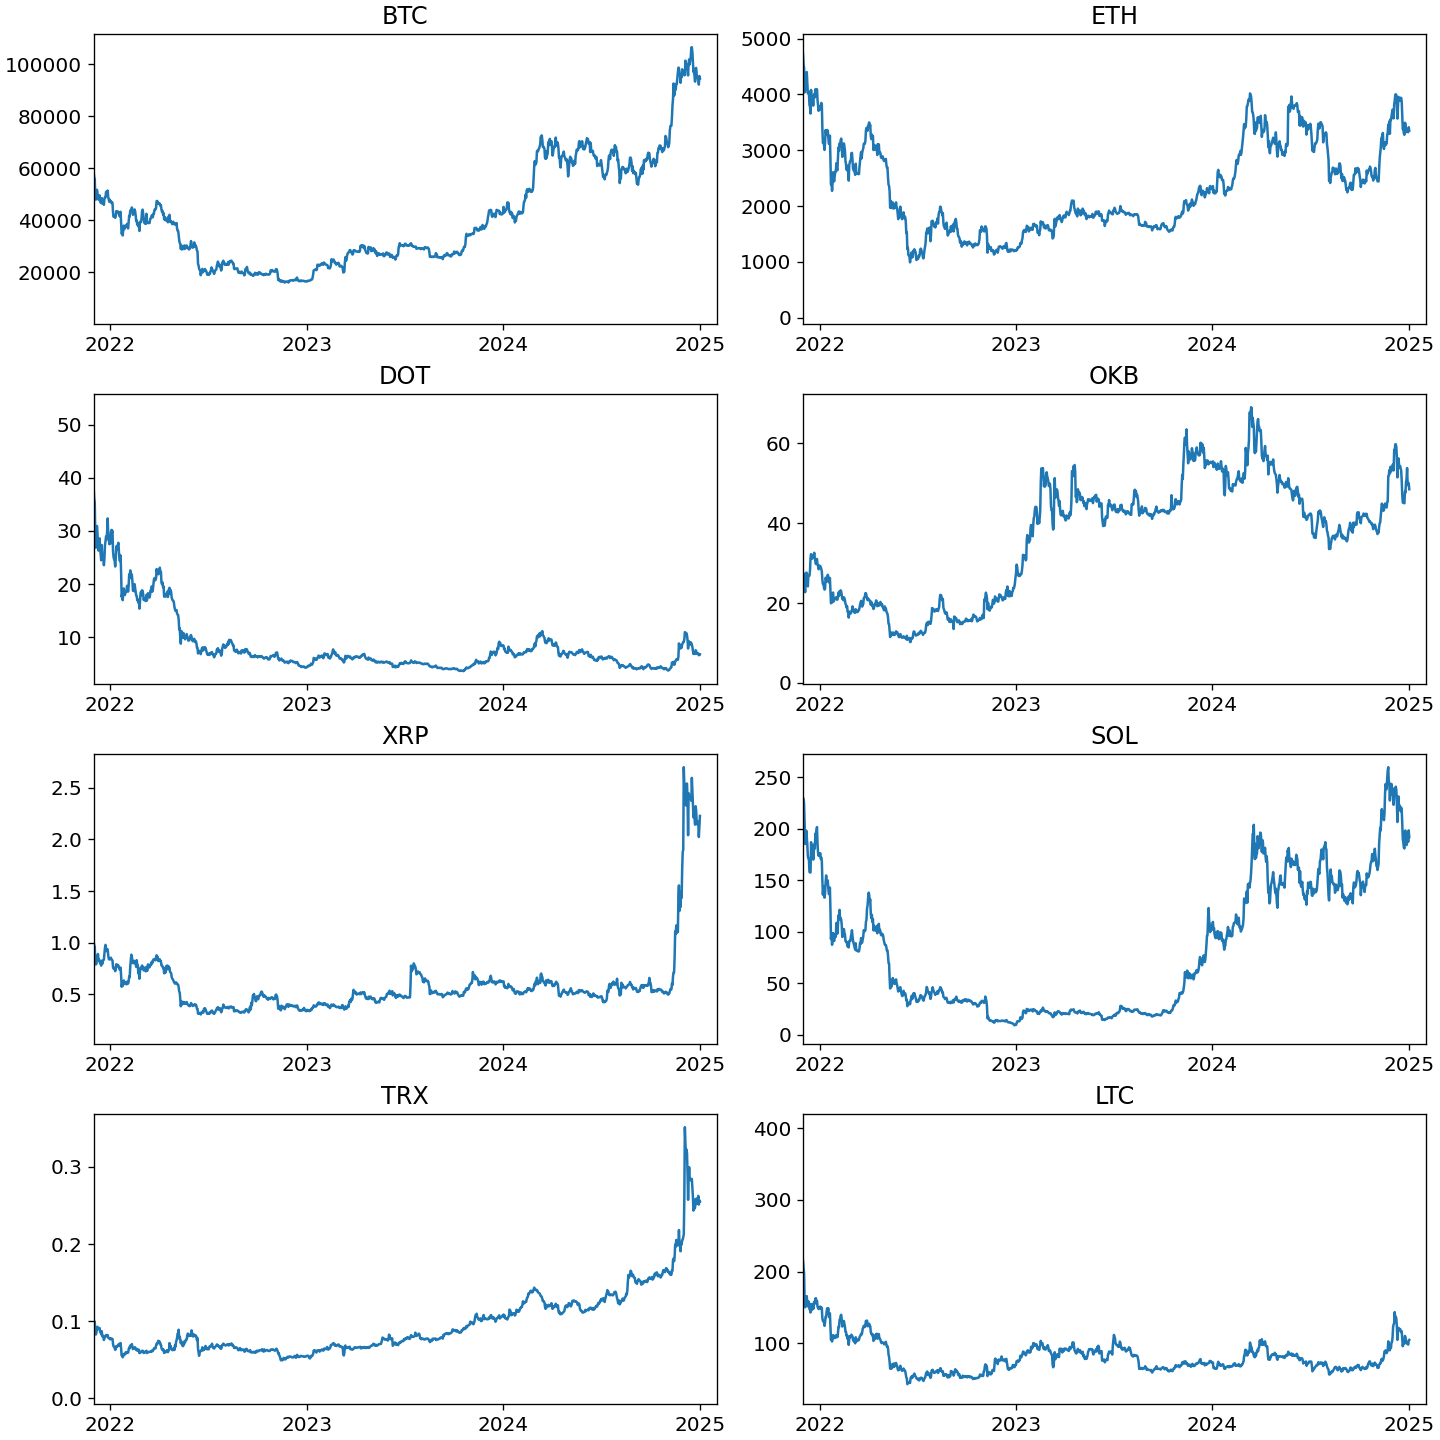
\includegraphics[width=1\textwidth]{prices.png}
                \caption{Цены активов}
                \label{fig:prices}
            \end{figure}
        \end{column}
        \begin{column}{0.5\textwidth}
            \begin{figure}
                \centering
                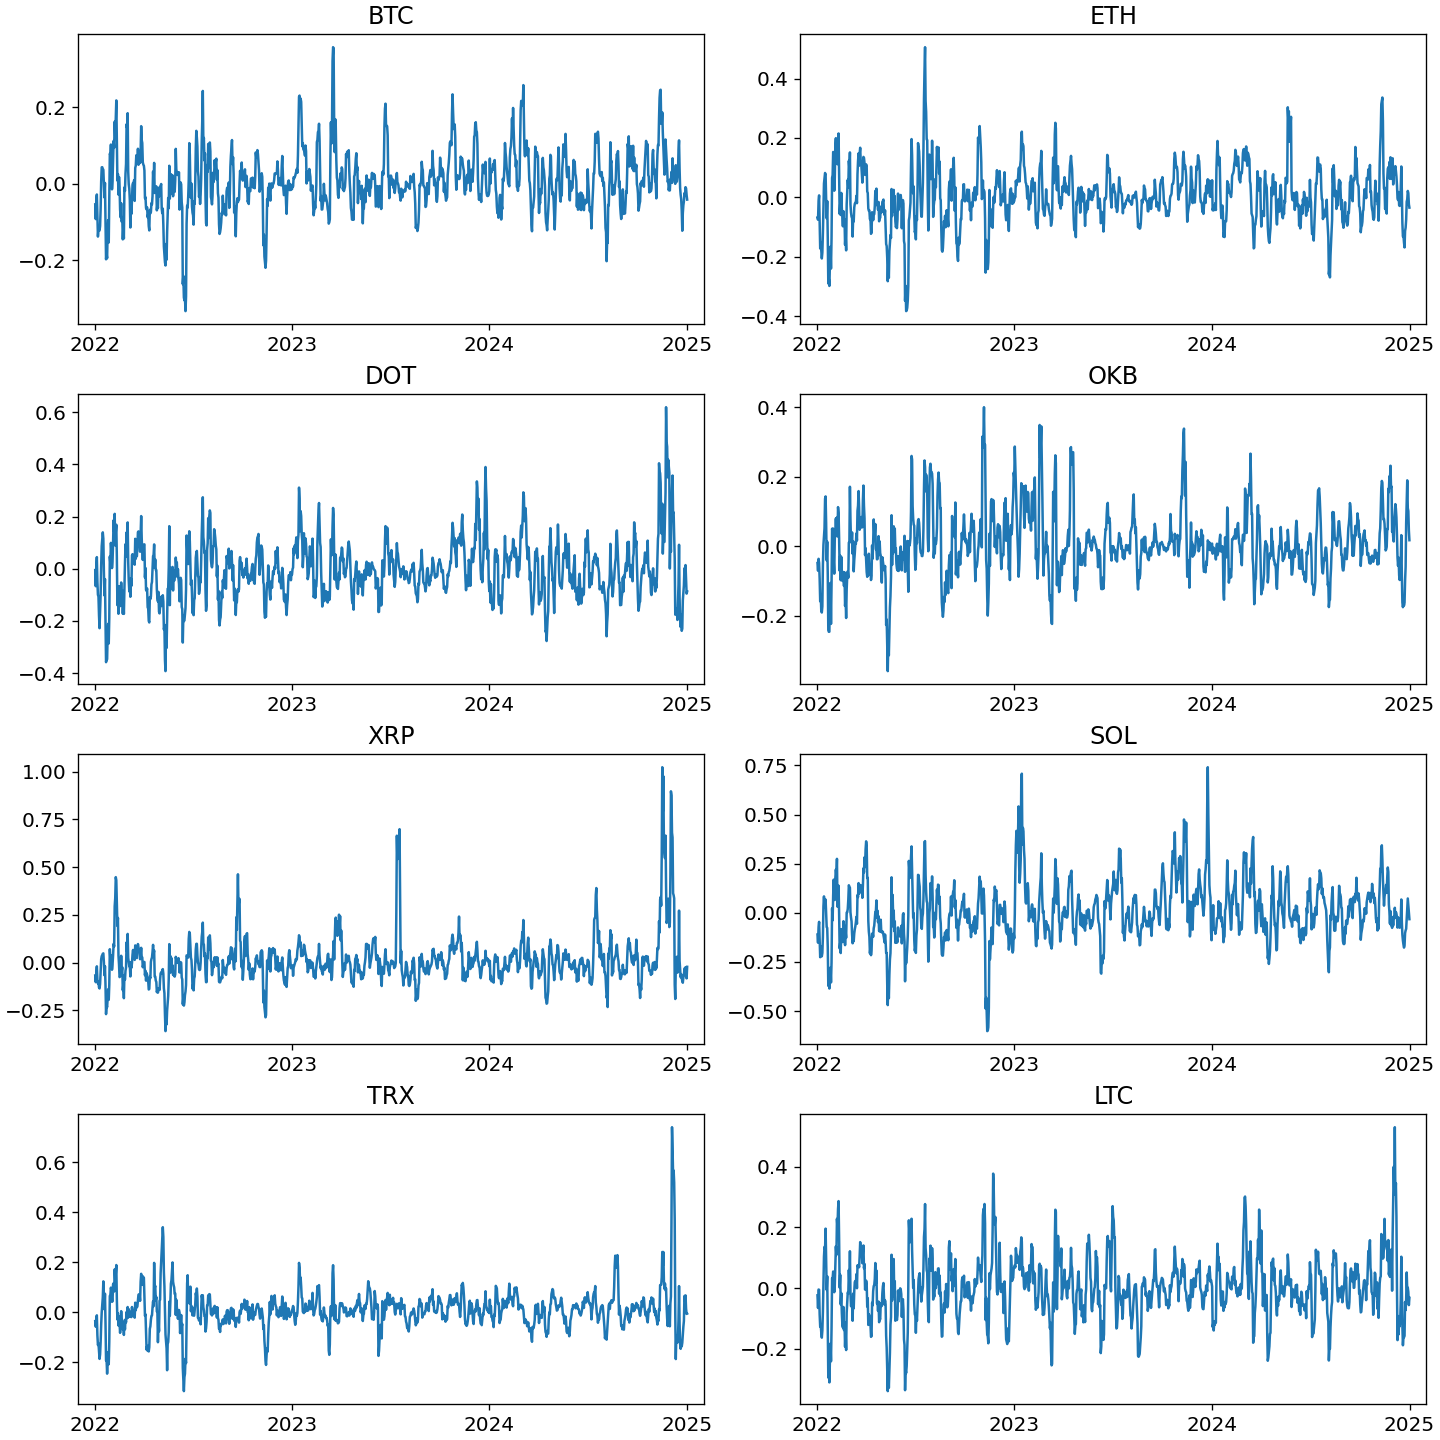
\includegraphics[width=1\textwidth]{returns.png}
                \caption{Доходности активов}
                \label{fig:returns}
            \end{figure}
        \end{column}
    \end{columns}
\end{frame}

\begin{frame}
    \frametitle{}
    \begin{table}[h]
        \caption{Доходности активов}
        \setlength{\tabcolsep}{3pt}
        \begin{tabularx}{\textwidth}{lrrrrrrrr}
            \toprule
            & BTC & ETH & DOT & OKB & XRP & SOL & TRX & LTC \\
            \midrule
            mean & 0.0073 & 0.0038 & -0.0031 & 0.0077 & 0.0132 & 0.0114 & 0.0105 & 0.0025 \\
            std & 0.0779 & 0.0961 & 0.1110 & 0.0936 & 0.1328 & 0.1482 & 0.0800 & 0.1001 \\
            min & -0.3328 & -0.3830 & -0.3925 & -0.3591 & -0.3596 & -0.6018 & -0.3162 & -0.3392 \\
            25\% & -0.0358 & -0.0477 & -0.0724 & -0.0401 & -0.0506 & -0.0765 & -0.0236 & -0.0513 \\
            50\% & 0.0026 & -0.0013 & -0.0084 & -0.0016 & -0.0003 & -0.0034 & 0.0106 & 0.0001 \\
            75\% & 0.0446 & 0.0555 & 0.0573 & 0.0494 & 0.0430 & 0.0906 & 0.0373 & 0.0546 \\
            max & 0.3566 & 0.5056 & 0.6188 & 0.4003 & 1.0235 & 0.7409 & 0.7407 & 0.5294 \\
            \bottomrule
        \end{tabularx}
        \label{tab:returns_describe}
    \end{table}
\end{frame}

\begin{frame}
    \frametitle{}
    \begin{figure}[H]
        \centering
        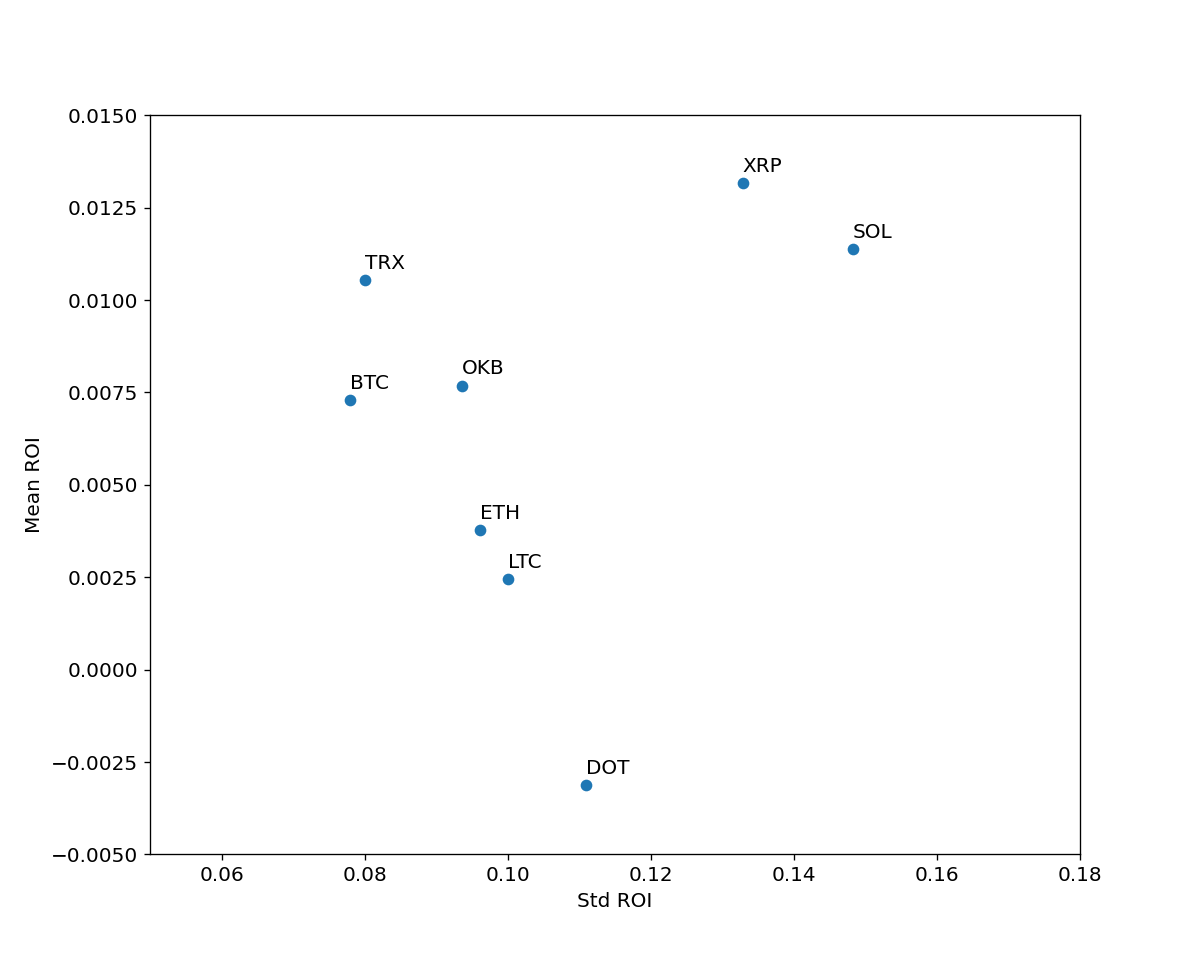
\includegraphics[width=0.9\textwidth]{rois_mean_std.png}
        \caption{Среднее и стандартное отклонение доходностей}
        \label{fig:rois_mean_std}
    \end{figure}
\end{frame}

\begin{frame}
    \frametitle{}
    \begin{figure}[H]
        \centering
        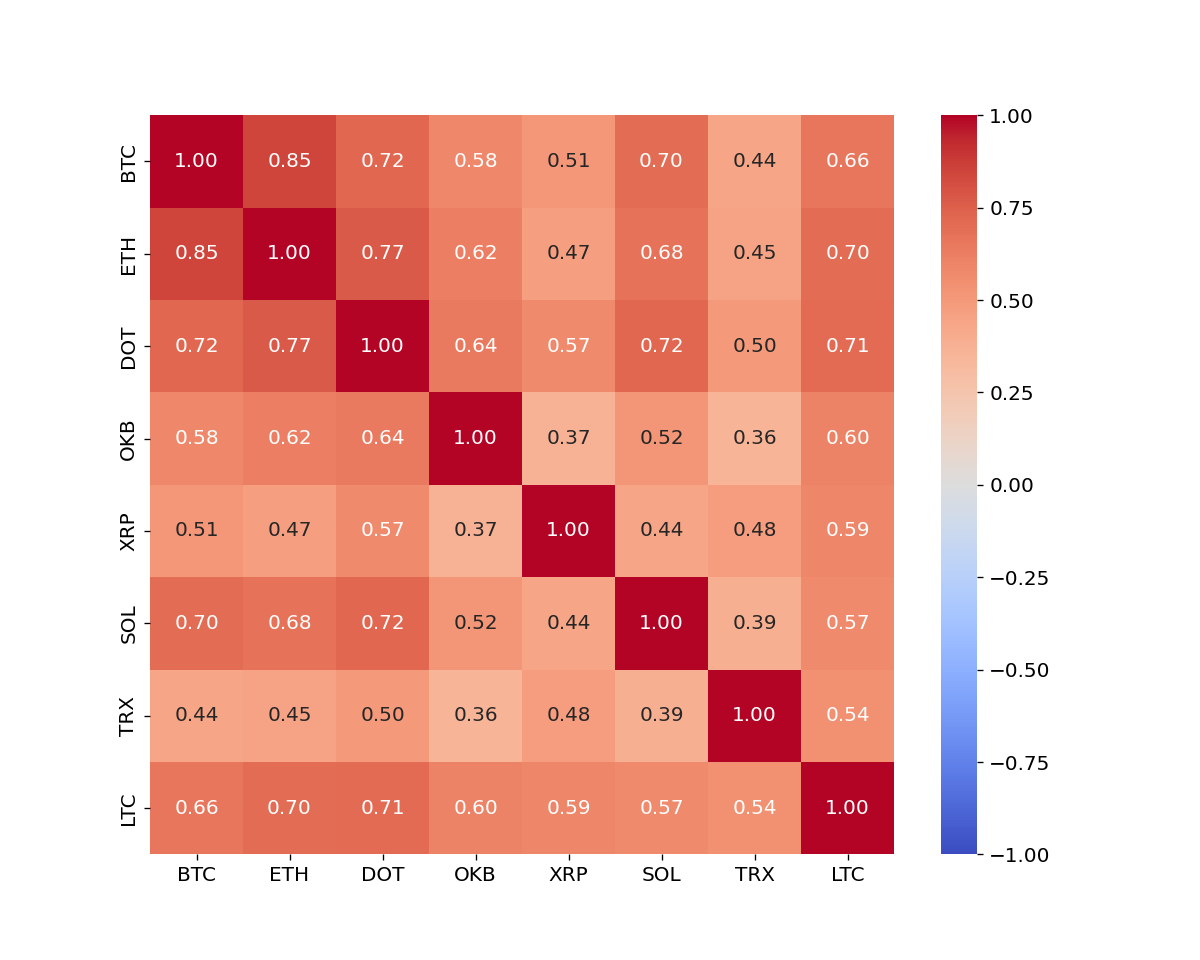
\includegraphics[width=0.9\textwidth]{corr.png}
        \caption{Корреляции доходностей активов}
        \label{fig:corr}
    \end{figure}
\end{frame}

\begin{frame}
    \frametitle{}
    Модели оценки средней доходности:
    \begin{enumerate}
        \item NAIVE --- среднее выборочное
        \item MARTINGAL --- последнее наблюдаемое
        \item ARIMA --- модель ARIMA
        \item LR --- линейная регрессия
        \item RF --- случайный лес
    \end{enumerate}

    Качество прогонозирования оценивается по метрике 
    \[
	MSE = \frac{1}{n} \sum_{i=1}^{n} (r_i - \hat{r}_i)^2
    \]
    где $r_i$ - истинное значение доходности,
    а $\hat{r}_i$ - прогнозное значение модели на $i$-м объекте тестовой выборки.
\end{frame}

\begin{frame}
    \begin{table}[h]
    \caption{Качество прогнозирования, MSE$\cdot 10^4$}
        \label{tab:ml_eval_metrics}
        \begin{tabular}{lrrrrr}
            \toprule
            & NAIVE & MARTINGAL & LR & ARIMA & RF \\
            \midrule
            BTC & 5.63 & 1.20 & 1.58 & 1.62 & 2.07 \\
            ETH & 8.00 & 1.99 & 4.47 & 3.70 & 5.05 \\
            DOT & 16.51 & 3.89 & 4.09 & 3.98 & 5.28 \\
            OKB & 6.06 & 1.56 & 1.77 & 1.95 & 2.05 \\
            XRP & 24.33 & 5.04 & 6.98 & 5.71 & 6.53 \\
            SOL & 21.19 & 4.47 & 11.86 & 6.16 & 5.31 \\
            TRX & 7.96 & 1.85 & 4.19 & 5.30 & 6.04 \\
            LTC & 8.53 & 2.66 & 2.24 & 3.22 & 5.11 \\
            \bottomrule
        \end{tabular}
    \end{table}
\end{frame}

\begin{frame}
    \frametitle{}
    Имея $r_t$ - вектор-столбец доходностей в момент времени t, по истории наблюдений $r_1, \cdots r_n$ 
    выборочная ковариация $\hat{\Sigma}$ рассчитывается как 
    \begin{align}
        \hat{\Sigma} = \frac{1}{n} \sum_{t=1}^{n}(r_t - \overline{r}) \cdot (r_t - \overline{r})^T
    \end{align}
    где $\overline{r} = \frac{1}{n} \sum_{t=1}^{n} r_t$.    
\end{frame}

\begin{frame}
    \frametitle{}
    \textbf{Стратегия} --- принцип по которому в каждый момент времени формируется портфель.

    Стратегии Марковица определяются моделью, лежащей в основе оценок $\hat{\mu}$ и $\hat{\Sigma}$,
    а так же зависят от параметра $\tau$.
    
    Тривиальные стратегии:
    \begin{enumerate}
        \item UNIFORM --- равномерное инвестирование во все активы
        \item MOST RISKY --- наиболее рискованный
        \item LESS RISKY --- наименее рискованный
        \item BEST RETURN --- с наибольшей доходностью
        \item WORST RETURN --- с наименьшей доходностью
    \end{enumerate}

    Доходность стратегии \textbf{ROI} (Return On Investment) определяется аналогично доходности портфеля.
\end{frame} 

\begin{frame}
    \frametitle{title}
    \begin{figure}
        \centering
        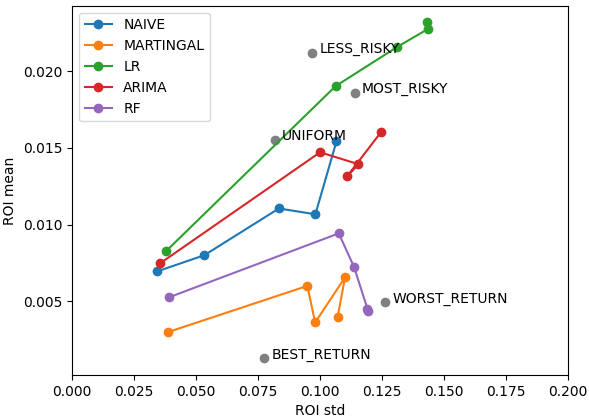
\includegraphics[width=0.9\textwidth]{result_frontiers_cut.png}
        \caption{Результаты тестирования стратегий}
        \label{fig:result_frontier}
    \end{figure}
\end{frame}

\begin{frame}
    \frametitle{}
    \begin{table}[H]
        \caption{Тривиальные портфели}
        \label{tab:trivial_rois}
        \begin{tabular}{lrr}
            \toprule
            & mean ROI $\cdot 10^3$ & std ROI $\cdot 10^2$ \\
            \midrule
            UNIFORM & 15.5372 & 8.1775 \\
            MOST RISKY & 18.5904 & 11.3970 \\
            LESS RISKY & 21.1635 & 9.6881 \\
            BEST RETURN & 1.2790 & 7.7329 \\
            WORST RETURN & 4.9217 & 12.6324 \\
            \bottomrule
        \end{tabular}
    \end{table}
\end{frame}

\begin{frame}
    \begin{table}[H]
        \caption{Средние ROI $\cdot 10^3$}
        \label{tab:roi_mean}
        \begin{tabular}{lrrrrr}
            \toprule
            &  0.01 &  0.25 &  0.50 &  0.75 &  1.00 \\
            \midrule
            NAIVE & 6.9451 & 8.0025 & 11.0462 & 10.6657 & 15.4227 \\
            MARTINGAL & 2.9859 & 6.0019 & 3.6178 & 6.5656 & 3.9942 \\
            LR & 8.2600 & 19.0185 & 21.5537 & 22.7442 & 23.1668 \\
            ARIMA & 7.4648 & 14.7066 & 13.9296 & 13.1520 & 15.9971 \\
            RF & 5.2633 & 9.4236 & 7.2398 & 4.3777 & 4.5050 \\
            \bottomrule
        \end{tabular}
    \end{table}
\end{frame}

\begin{frame}
    \begin{table}[H]
        \caption{Стандартное отклонение ROI $\cdot 10^2$}
        \label{tab:roi_std}
        \begin{tabular}{lrrrrr}
            \toprule
            &  0.01 &  0.25 &  0.50 &  0.75 &  1.00 \\
            \midrule
            NAIVE & 3.4328 & 5.3375 & 8.3427 & 9.8131 & 10.6650 \\
            MARTINGAL & 3.8577 & 9.4886 & 9.8051 & 11.0111 & 10.7128 \\
            LR & 3.7892 & 10.6314 & 13.1000 & 14.3570 & 14.3071 \\
            ARIMA & 3.5454 & 10.0037 & 11.5506 & 11.1001 & 12.4518 \\
            RF & 3.9215 & 10.7564 & 11.3710 & 11.9397 & 11.9118 \\
            \bottomrule
        \end{tabular}
    \end{table}
\end{frame}

\section{Результаты}

\begin{frame}
    Выводы:
    \begin{itemize}
        \item активы имеют сильную положительную корреляцию
        \item стремление сформировать портфель с большей доходностью влечет большие риски
        \item диверсификация действительно позволяет снижать риск портфеля
        \item как правило, формирование портфеля доминирует над инвестированием в отдельные активы
        \item линейная модель авторегрессии показала лучшее качество для оценки средней доходности
    \end{itemize}
\end{frame}

\begin{frame}
    \frametitle{}
    Дальнейшие шаги по исследованию данной темы:
    \begin{itemize}
        \item рассмотреть другие классы методов прогнозирования временных рядов
        \item помимо авторегрессионных признаков, учесть влияние внешних факторов на формирование цен
        \item расширить рассматриваемый набор активов
        \item исследовать другие таймфреймы и периоды инвестирования
    \end{itemize}
\end{frame}

\begin{frame}
    \centering
    Спасибо за внимание.
\end{frame}

\end{document}